\documentclass[12pt,a4paper]{article}%
\usepackage[T1]{fontenc}%
\usepackage[utf8]{inputenc}%
\usepackage{lmodern}%
\usepackage{textcomp}%
\usepackage{lastpage}%
\usepackage{ulem}%
\usepackage[HTML]{xcolor}%
\usepackage{soul}%
\usepackage{ifthen}%
\usepackage{fancyhdr}%
\usepackage{tikz}%
\usepackage{unicode-math}%
\usepackage{fontspec}%
\usepackage{ragged2e}%
%
\usepackage{geometry}%
\geometry{top=49mm, bottom=25mm, outer=10mm, inner=24mm}%
\usepackage{graphicx}%
\usepackage{eso-pic}%
\usepackage{tcolorbox}%
\usepackage{inputenc}%

            \pagestyle{fancy}
            \fancyhf{} % Clear existing headers and footers
            \fancyhead{} % Clear the header
            \fancyfoot[C]{% Centered footer
                \mbox{\tikz[baseline=(page.base)]{
                    \node[draw=black, fill=white, rounded corners=3pt, inner sep=3pt] (page) {\thepage};
                }}
            }
            \renewcommand{\headrulewidth}{0pt} % Remove the top black line
            \renewcommand{\footrulewidth}{0pt} % Remove any footer line
            %

    \newcommand\OddBackgroundPic{
        \put(0,0){%
            \parbox[b][\paperheight]{\paperwidth}{%
                \vfill
                \centering
                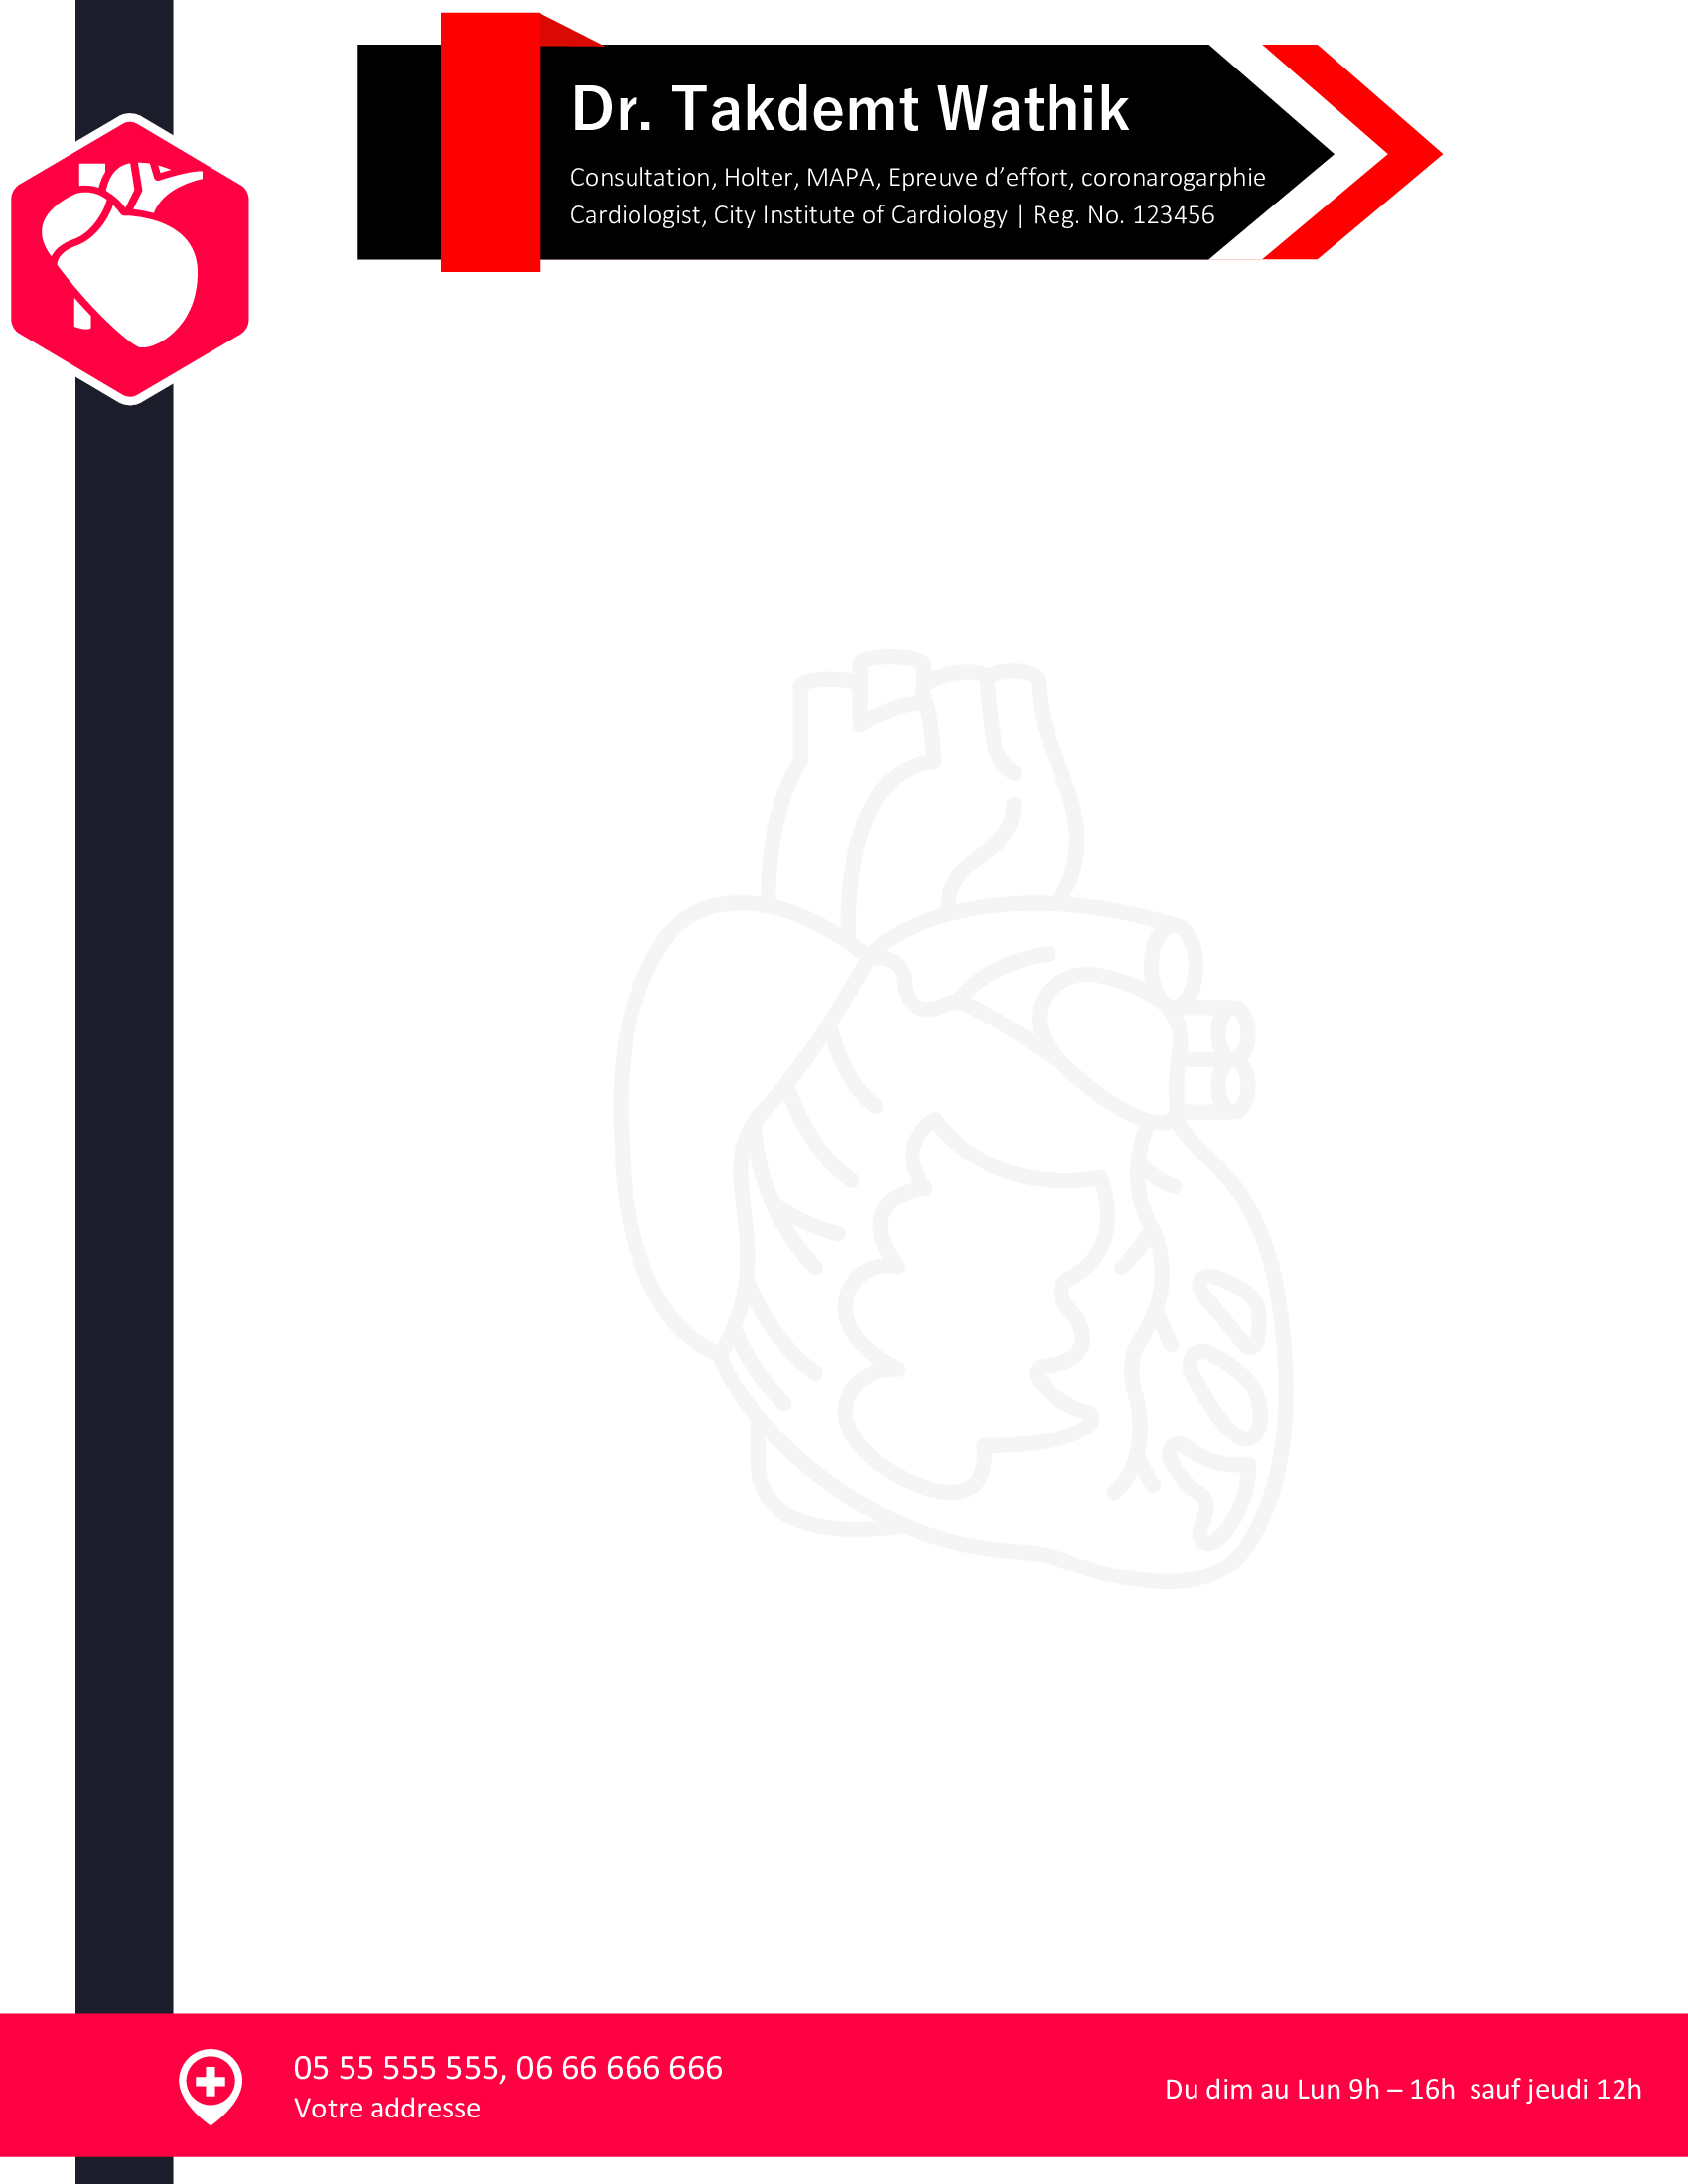
\includegraphics[width=\paperwidth,height=\paperheight]{/home/mac/boltStation/pythonBackend/Templates/1withHeader.jpg}
                \vfill
            }
        }
    }
    %

    \newcommand\EvenBackgroundPic{
        \put(0,0){%
            \parbox[b][\paperheight]{\paperwidth}{%
                \vfill
                \centering
                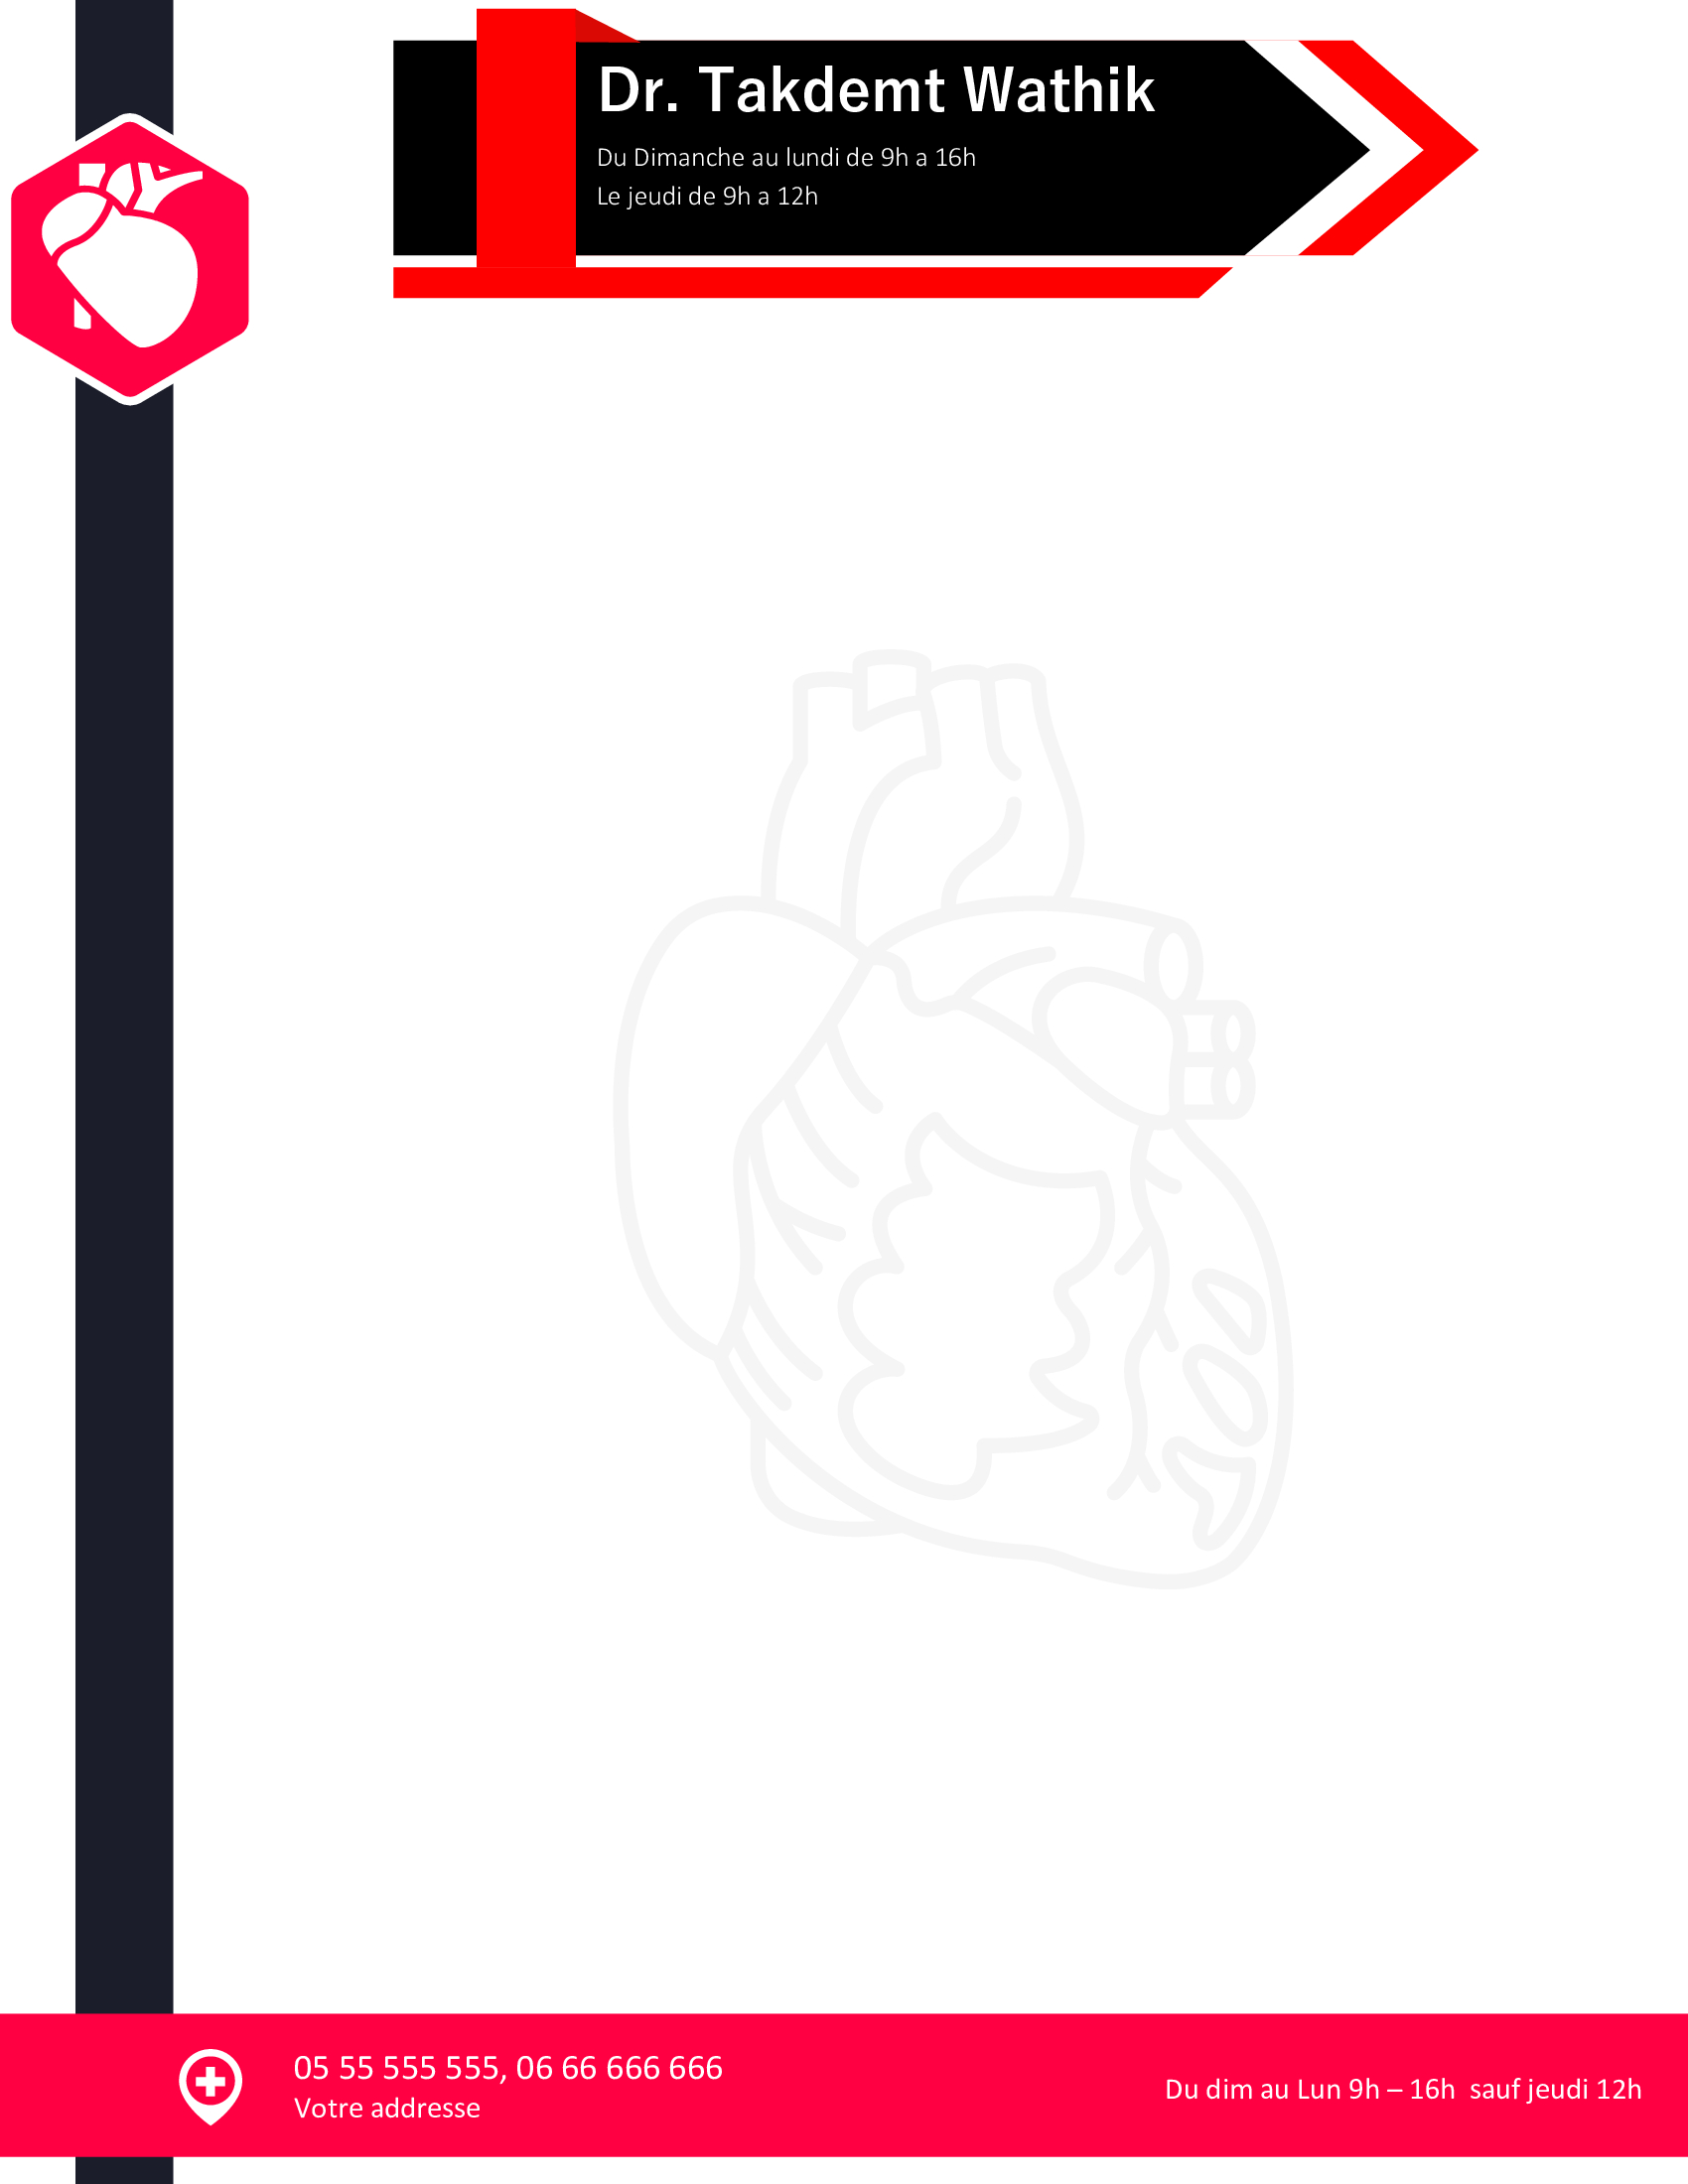
\includegraphics[width=\paperwidth,height=\paperheight]{/home/mac/boltStation/pythonBackend/Templates/1noHeader.jpg}
                \vfill
            }
        }
    }
    %

    \AddToShipoutPictureBG{%
        \ifthenelse{\isodd{\value{page}}}{\OddBackgroundPic}{\EvenBackgroundPic}%
    }
    %
\definecolor{main_title_background_color}{HTML}{e2e8f0}%
\definecolor{main_title_border_color}{HTML}{1e293b}%
\definecolor{kinetic_base_color}{HTML}{f1f5f9}%
\definecolor{hypokinetic_color}{HTML}{fecdd3}%
\definecolor{akinetic_color}{HTML}{f87171}%
\definecolor{dyskinetic_color}{HTML}{fcd34d}%
%
\begin{document}%
\normalsize%
\begin{minipage}{0.5\linewidth}%
\textbf{\underline{Nom :}} \hspace{1cm} Zighoud%
\\%
\textbf{\underline{Prénom :}} \hspace{1cm} Sabine%
\\%
\end{minipage}%
\begin{minipage}{0.5\linewidth}%
\textbf{\underline{DDN :}} \hspace{1cm} 26-08-1991%
\\%
\textbf{\underline{Date :}} \hspace{1cm} 30/12/2024%
\\%
\end{minipage}%
\hspace{\textwidth}%
\\%
\begin{center}%

            \begin{tcolorbox}[
                colframe=main_title_border_color,        % Couleur de la bordure
                colback=main_title_background_color,        % Couleur de fond
                coltitle=main_title_border_color,       % Couleur du texte (si titre utilisé)
                arc=8pt,              % Rayon des coins arrondis
                boxrule=0.5mm,          % Épaisseur de la bordure
                auto outer arc,       % Ajuste automatiquement les coins arrondis
                width=\linewidth,     % Largeur de la boîte
                halign=center         % Centrer le texte horizontalement
            ]
            \LARGE{\textbf{Echocardiographie}}
            \end{tcolorbox}
            %
\end{center}%
%
\vspace*{\baselineskip}%
\textbf{\ul{Cinètique du VG:}}%
\\%
Akinesie interessant 6 segments dans le territoire inferieur dans ses trois segments basal median et apical, infero{-}lateral dans ses deux segments basal et median, latero{-}apical. Hypokinesie interessant 5 segments dans le territoire inferieur dans ses trois segments basal median et apical, infero{-}septal dans ses deux segments basal et median. Dyskinesie interessant 5 segments dans le territoire anterieur dans ses trois segments basal median et apical, antero{-}lateral dans ses deux segments basal et median.%
\\%
\\%
\begin{minipage}{1.0\linewidth}%
\def \globalscale {0.50000}%
\centering%
		
		\begin{tikzpicture}[y=1cm, x=1cm, yscale=\globalscale,xscale=\globalscale, every node/.append style={scale=\globalscale}, inner sep=0pt, outer sep=0pt]
			
			\begin{scope}[even odd rule,line join=round,miter limit=2.0,shift={(-3.1277, 6.0325)}]
				\path[fill=kinetic_base_color,even odd rule,line join=round,miter limit=2.0] (5.307, 2.1032).. controls (5.307, 2.1032) and (5.5352, 2.2407) .. (5.5878, 2.2627).. controls (5.6404, 2.2848) and (6.0546, 2.4708) .. (6.1757, 2.5093).. controls (6.2967, 2.5477) and (6.6448, 2.6506) .. (6.8003, 2.6744).. controls (6.9558, 2.6981) and (7.1993, 2.7206) .. (7.4564, 2.7247).. controls (7.7135, 2.7287) and (8.1244, 2.7098) .. (8.4259, 2.6382).. controls (8.7275, 2.5666) and (9.0519, 2.4595) .. (9.3367, 2.3242).. controls (9.6215, 2.1888) and (9.7334, 2.1255) .. (9.8043, 2.0807).. controls (9.7225, 1.9675) and (9.6791, 1.8926) .. (9.5649, 1.7294).. controls (9.4508, 1.5663) and (9.442, 1.5516) .. (9.3221, 1.3718).. controls (9.2023, 1.1919) and (9.1932, 1.1836) .. (9.1932, 1.1805).. controls (9.0537, 1.2613) and (8.8777, 1.3772) .. (8.7349, 1.4454).. controls (8.6001, 1.5098) and (8.1245, 1.6922) .. (7.7331, 1.7098).. controls (7.3373, 1.7276) and (6.7883, 1.6216) .. (6.6824, 1.5891).. controls (6.5766, 1.5566) and (6.3873, 1.4945) .. (6.2374, 1.4235).. controls (6.0876, 1.3526) and (5.9221, 1.2687) .. (5.8337, 1.2058).. controls (5.7452, 1.3161) and (5.307, 2.1032) .. (5.307, 2.1032) -- cycle;
				
				
				
				\path[fill,even odd rule,line join=round,miter limit=2.0] (5.307, 2.1032).. controls (5.307, 2.1032) and (5.5352, 2.2407) .. (5.5878, 2.2627).. controls (5.6404, 2.2848) and (6.0546, 2.4708) .. (6.1757, 2.5093).. controls (6.2967, 2.5477) and (6.6448, 2.6506) .. (6.8003, 2.6744).. controls (6.9558, 2.6981) and (7.1993, 2.7206) .. (7.4564, 2.7247).. controls (7.7135, 2.7287) and (8.1244, 2.7098) .. (8.4259, 2.6382).. controls (8.7275, 2.5666) and (9.0519, 2.4595) .. (9.3367, 2.3242).. controls (9.6215, 2.1888) and (9.7334, 2.1255) .. (9.8043, 2.0807).. controls (9.7225, 1.9675) and (9.6791, 1.8926) .. (9.5649, 1.7294).. controls (9.4508, 1.5663) and (9.442, 1.5516) .. (9.3221, 1.3718).. controls (9.2023, 1.1919) and (9.1932, 1.1836) .. (9.1932, 1.1805).. controls (9.0537, 1.2613) and (8.8777, 1.3772) .. (8.7349, 1.4454).. controls (8.6001, 1.5098) and (8.1245, 1.6922) .. (7.7331, 1.7098).. controls (7.3373, 1.7276) and (6.7883, 1.6216) .. (6.6824, 1.5891).. controls (6.5766, 1.5566) and (6.3873, 1.4945) .. (6.2374, 1.4235).. controls (6.0876, 1.3526) and (5.9221, 1.2687) .. (5.8337, 1.2058).. controls (5.7452, 1.3161) and (5.307, 2.1032) .. (5.307, 2.1032) -- cycle(9.1771, 1.2514).. controls (9.1958, 1.2787) and (9.2269, 1.3243) .. (9.2781, 1.4011).. controls (9.3983, 1.5815) and (9.4071, 1.5962) .. (9.5216, 1.7598).. controls (9.6196, 1.8998) and (9.6655, 1.975) .. (9.7283, 2.065).. controls (9.6551, 2.1079) and (9.5393, 2.1693) .. (9.314, 2.2764).. controls (9.0325, 2.4102) and (8.7118, 2.5159) .. (8.4137, 2.5867).. controls (8.1162, 2.6574) and (7.7108, 2.6758) .. (7.4573, 2.6718).. controls (7.203, 2.6677) and (6.9621, 2.6455) .. (6.8083, 2.622).. controls (6.6547, 2.5986) and (6.3112, 2.4968) .. (6.1917, 2.4588).. controls (6.0716, 2.4206) and (5.6605, 2.2358) .. (5.6083, 2.214).. controls (5.5713, 2.1984) and (5.4457, 2.1245) .. (5.3782, 2.0841).. controls (5.4628, 1.9327) and (5.7396, 1.4399) .. (5.8471, 1.2782).. controls (5.942, 1.3378) and (6.0841, 1.4095) .. (6.2148, 1.4714).. controls (6.3671, 1.5434) and (6.5594, 1.6067) .. (6.6669, 1.6397).. controls (6.7746, 1.6727) and (7.3329, 1.7808) .. (7.7355, 1.7627).. controls (8.1349, 1.7447) and (8.6201, 1.5589) .. (8.7577, 1.4932).. controls (8.8874, 1.4312) and (9.0444, 1.3303) .. (9.1771, 1.2514) -- cycle;
				
				
				
				\path[fill=kinetic_base_color,even odd rule,line join=round,miter limit=2.0] (5.2642, 2.0803).. controls (5.2298, 2.0551) and (4.8854, 1.8472) .. (4.7698, 1.7201).. controls (4.6542, 1.593) and (4.0075, 1.0579) .. (3.7281, 0.5261).. controls (3.4965, 0.0851) and (3.4862, 0.1466) .. (3.3821, -0.1767).. controls (3.1956, -0.756) and (3.2271, -0.5781) .. (3.1637, -1.0521).. controls (3.1132, -1.4292) and (3.1573, -1.4911) .. (3.1573, -1.4911).. controls (3.3896, -1.4942) and (4.2675, -1.512) .. (4.2675, -1.512).. controls (4.2702, -1.3422) and (4.3243, -0.4839) .. (4.6056, -0.0878).. controls (4.8869, 0.3082) and (5.2094, 0.7609) .. (5.8141, 1.1786).. controls (5.5641, 1.5793) and (5.3131, 2.0487) .. (5.3131, 2.0487).. controls (5.3018, 2.0626) and (5.2985, 2.1055) .. (5.2642, 2.0803) -- cycle;
				
				
				
				\path[fill,even odd rule,line join=round,miter limit=2.0] (3.2102, -1.4919).. controls (3.2102, -1.4917) and (3.2102, -1.4916) .. (3.2102, -1.4915).. controls (3.2103, -1.4819) and (3.2078, -1.4728) .. (3.2034, -1.4651).. controls (3.2034, -1.4653) and (3.2035, -1.4654) .. (3.2035, -1.4654) -- (3.2009, -1.4611) -- (3.1849, -1.4915).. controls (3.1749, -1.4913) and (3.1657, -1.4912) .. (3.1573, -1.4911).. controls (3.1573, -1.4911) and (3.1132, -1.4292) .. (3.1637, -1.0521).. controls (3.2271, -0.5781) and (3.1956, -0.756) .. (3.3821, -0.1767).. controls (3.4862, 0.1466) and (3.4965, 0.0851) .. (3.7281, 0.5261).. controls (4.0075, 1.0579) and (4.6542, 1.593) .. (4.7698, 1.7201).. controls (4.8854, 1.8472) and (5.2298, 2.0551) .. (5.2642, 2.0803).. controls (5.2985, 2.1055) and (5.3018, 2.0626) .. (5.3131, 2.0487).. controls (5.3131, 2.0487) and (5.5641, 1.5793) .. (5.8141, 1.1786).. controls (5.2094, 0.7609) and (4.8869, 0.3082) .. (4.6056, -0.0878).. controls (4.3243, -0.4839) and (4.2702, -1.3422) .. (4.2675, -1.512).. controls (4.2675, -1.512) and (3.4997, -1.4965) .. (3.2102, -1.4919) -- cycle(3.1984, -1.4388).. controls (3.4344, -1.4424) and (4.0355, -1.4544) .. (4.2164, -1.458).. controls (4.2279, -1.2034) and (4.2977, -0.4301) .. (4.5624, -0.0572).. controls (4.8402, 0.3339) and (5.1582, 0.7793) .. (5.7428, 1.1932).. controls (5.5144, 1.5635) and (5.2925, 1.9753) .. (5.2686, 2.0198).. controls (5.1785, 1.962) and (4.908, 1.7934) .. (4.809, 1.6845).. controls (4.6943, 1.5584) and (4.052, 1.0288) .. (3.775, 0.5015).. controls (3.546, 0.0656) and (3.5354, 0.1266) .. (3.4325, -0.1929).. controls (3.2479, -0.7662) and (3.2789, -0.59) .. (3.2161, -1.0591).. controls (3.1862, -1.2825) and (3.1923, -1.3931) .. (3.1984, -1.4388) -- cycle;
				
				
				
				\path[fill=kinetic_base_color,even odd rule,line join=round,miter limit=2.0] (3.1334, -1.5182).. controls (3.1334, -1.5182) and (3.0928, -2.0672) .. (3.2278, -2.6289).. controls (3.3295, -3.0522) and (3.705, -3.8756) .. (4.0259, -4.276).. controls (4.3491, -4.6794) and (4.9149, -5.2073) .. (4.9149, -5.2073).. controls (5.5392, -4.3026) and (5.5633, -4.2174) .. (5.5633, -4.2174).. controls (5.5633, -4.2174) and (5.2539, -3.9496) .. (5.1407, -3.7904).. controls (5.0275, -3.6312) and (4.4521, -2.7653) .. (4.3771, -2.3298).. controls (4.2991, -1.8776) and (4.2664, -1.5338) .. (4.2664, -1.5338).. controls (3.9492, -1.5468) and (3.1334, -1.5182) .. (3.1334, -1.5182) -- cycle;
				
				
				
				\path[fill,even odd rule,line join=round,miter limit=2.0] (3.1334, -1.5182).. controls (3.1334, -1.5182) and (3.9492, -1.5468) .. (4.2664, -1.5338).. controls (4.2664, -1.5338) and (4.2991, -1.8776) .. (4.3771, -2.3298).. controls (4.4521, -2.7653) and (5.0275, -3.6312) .. (5.1407, -3.7904).. controls (5.2539, -3.9496) and (5.5633, -4.2174) .. (5.5633, -4.2174).. controls (5.5633, -4.2174) and (5.5392, -4.3026) .. (4.9149, -5.2073).. controls (4.9149, -5.2073) and (4.3491, -4.6794) .. (4.0259, -4.276).. controls (3.705, -3.8756) and (3.3295, -3.0522) .. (3.2278, -2.6289).. controls (3.0928, -2.0672) and (3.1334, -1.5182) .. (3.1334, -1.5182) -- cycle(5.497, -4.2294).. controls (5.414, -4.1556) and (5.1908, -3.9521) .. (5.0976, -3.8211).. controls (4.9827, -3.6596) and (4.4011, -2.7805) .. (4.3249, -2.3388).. controls (4.2641, -1.9862) and (4.2307, -1.6992) .. (4.2188, -1.5883).. controls (3.9279, -1.5956) and (3.3579, -1.5785) .. (3.1835, -1.5728).. controls (3.1774, -1.7197) and (3.1704, -2.164) .. (3.2792, -2.6165).. controls (3.3797, -3.0345) and (3.7504, -3.8476) .. (4.0672, -4.2429).. controls (4.334, -4.5759) and (4.7671, -4.9941) .. (4.9064, -5.1264).. controls (5.3137, -4.5348) and (5.4543, -4.3036) .. (5.497, -4.2294) -- cycle;
				
				
				
				\path[fill=akinetic_color,even odd rule,line join=round,miter limit=2.0] (4.9689, -5.2263).. controls (5.1642, -5.3422) and (6.0373, -5.918) .. (6.8234, -5.9993).. controls (7.6095, -6.0807) and (8.5796, -5.9881) .. (8.9477, -5.8401).. controls (9.3158, -5.692) and (9.7657, -5.4342) .. (9.7657, -5.4342).. controls (9.6201, -5.16) and (9.1626, -4.3867) .. (9.1626, -4.3867).. controls (8.9659, -4.5072) and (8.6311, -4.7019) .. (8.0379, -4.7978).. controls (7.4446, -4.8938) and (6.8534, -4.832) .. (6.5592, -4.72).. controls (6.265, -4.6079) and (5.5943, -4.2346) .. (5.5943, -4.2346).. controls (5.4804, -4.409) and (5.3934, -4.5397) .. (5.3934, -4.5397).. controls (5.3934, -4.5397) and (5.0372, -5.1011) .. (4.9689, -5.2263) -- cycle;
				
				
				
				\path[fill,even odd rule,line join=round,miter limit=2.0] (4.9689, -5.2263).. controls (5.0372, -5.1011) and (5.3934, -4.5397) .. (5.3934, -4.5397).. controls (5.3934, -4.5397) and (5.4804, -4.409) .. (5.5943, -4.2346).. controls (5.5943, -4.2346) and (6.265, -4.6079) .. (6.5592, -4.72).. controls (6.8534, -4.832) and (7.4446, -4.8938) .. (8.0379, -4.7978).. controls (8.6311, -4.7019) and (8.9659, -4.5072) .. (9.1626, -4.3867).. controls (9.1626, -4.3867) and (9.6201, -5.16) .. (9.7657, -5.4342).. controls (9.7657, -5.4342) and (9.3158, -5.692) .. (8.9477, -5.8401).. controls (8.5796, -5.9881) and (7.6095, -6.0807) .. (6.8234, -5.9993).. controls (6.0373, -5.918) and (5.1642, -5.3422) .. (4.9689, -5.2263) -- cycle(5.0404, -5.2078).. controls (5.2978, -5.3657) and (6.1008, -5.8714) .. (6.8288, -5.9467).. controls (7.6056, -6.027) and (8.5642, -5.9373) .. (8.9279, -5.791).. controls (9.2236, -5.6721) and (9.5724, -5.4818) .. (9.6945, -5.4136).. controls (9.5541, -5.1561) and (9.2387, -4.6198) .. (9.1443, -4.4597).. controls (8.9392, -4.5827) and (8.6058, -4.7596) .. (8.0463, -4.8501).. controls (7.4421, -4.9478) and (6.84, -4.8835) .. (6.5404, -4.7694).. controls (6.2892, -4.6737) and (5.7652, -4.389) .. (5.6117, -4.3047).. controls (5.515, -4.4524) and (5.4432, -4.5605) .. (5.4378, -4.5686).. controls (5.4264, -4.5865) and (5.1427, -5.0339) .. (5.0404, -5.2078) -- cycle;
				
				
				
				\path[fill=akinetic_color,even odd rule,line join=round,miter limit=2.0] (9.7863, -5.408).. controls (9.7863, -5.408) and (10.8486, -4.5998) .. (11.1878, -4.0579).. controls (11.4984, -3.5618) and (11.7079, -3.0625) .. (11.8125, -2.509).. controls (11.9025, -2.0323) and (11.8973, -1.5835) .. (11.8973, -1.5835).. controls (11.5718, -1.5775) and (10.7229, -1.5776) .. (10.7229, -1.5776).. controls (10.7145, -1.8423) and (10.5494, -2.7583) .. (10.27, -3.2237).. controls (9.9953, -3.6815) and (9.7193, -3.9361) .. (9.4396, -4.1741).. controls (9.3007, -4.2923) and (9.1878, -4.3672) .. (9.1878, -4.3672).. controls (9.3474, -4.6484) and (9.7863, -5.408) .. (9.7863, -5.408) -- cycle;
				
				
				
				\path[fill,even odd rule,line join=round,miter limit=2.0] (9.7863, -5.408).. controls (9.7863, -5.408) and (9.3474, -4.6484) .. (9.1878, -4.3672).. controls (9.1878, -4.3672) and (9.3007, -4.2923) .. (9.4396, -4.1741).. controls (9.7193, -3.9361) and (9.9953, -3.6815) .. (10.27, -3.2237).. controls (10.5494, -2.7583) and (10.7145, -1.8423) .. (10.7229, -1.5776).. controls (10.7229, -1.5776) and (11.5718, -1.5775) .. (11.8973, -1.5835).. controls (11.8973, -1.5835) and (11.9025, -2.0323) .. (11.8125, -2.509).. controls (11.7079, -3.0625) and (11.4984, -3.5618) .. (11.1878, -4.0579).. controls (10.8486, -4.5998) and (9.7863, -5.408) .. (9.7863, -5.408) -- cycle(9.8019, -5.3292).. controls (10.0109, -5.1665) and (10.8499, -4.4981) .. (11.143, -4.0299).. controls (11.4499, -3.5395) and (11.6572, -3.0462) .. (11.7605, -2.4992).. controls (11.8314, -2.1236) and (11.8425, -1.7655) .. (11.8441, -1.6356).. controls (11.5435, -1.6312) and (10.9486, -1.6306) .. (10.7729, -1.6305).. controls (10.7481, -1.951) and (10.5832, -2.8048) .. (10.3154, -3.251).. controls (10.037, -3.715) and (9.7574, -3.9731) .. (9.4739, -4.2144).. controls (9.3833, -4.2915) and (9.3034, -4.3506) .. (9.2577, -4.3831).. controls (9.4039, -4.6397) and (9.7056, -5.1624) .. (9.8019, -5.3292) -- cycle;
				
				
				
				\path[fill=kinetic_base_color,even odd rule,line join=round,miter limit=2.0] (8.2155, -0.887).. controls (8.2155, -0.887) and (7.9588, -0.6088) .. (7.6282, -0.6008).. controls (7.2976, -0.5929) and (7.2837, -0.6001) .. (7.0439, -0.6994).. controls (6.8915, -0.7625) and (6.8126, -0.8682) .. (6.8126, -0.8682).. controls (6.6907, -0.7511) and (6.1058, -0.1002) .. (6.1058, -0.1002).. controls (6.2224, 0.0035) and (6.4974, 0.2612) .. (6.848, 0.3598).. controls (7.1817, 0.4537) and (7.4679, 0.436) .. (7.7893, 0.3903).. controls (8.1107, 0.3446) and (8.3219, 0.2856) .. (8.5002, 0.1447).. controls (8.6784, 0.0038) and (8.9084, -0.2196) .. (8.9084, -0.2196).. controls (8.8151, -0.3121) and (8.2155, -0.887) .. (8.2155, -0.887) -- cycle;
				
				
				
				\path[fill,even odd rule,line join=round,miter limit=2.0] (8.2155, -0.887).. controls (8.2155, -0.887) and (7.9588, -0.6088) .. (7.6282, -0.6008).. controls (7.2976, -0.5929) and (7.2837, -0.6001) .. (7.0439, -0.6994).. controls (6.8915, -0.7625) and (6.8126, -0.8682) .. (6.8126, -0.8682).. controls (6.6907, -0.7511) and (6.1058, -0.1002) .. (6.1058, -0.1002).. controls (6.2224, 0.0035) and (6.4974, 0.2612) .. (6.848, 0.3598).. controls (7.1817, 0.4537) and (7.4679, 0.436) .. (7.7893, 0.3903).. controls (8.1107, 0.3446) and (8.3219, 0.2856) .. (8.5002, 0.1447).. controls (8.6784, 0.0038) and (8.9084, -0.2196) .. (8.9084, -0.2196).. controls (8.8151, -0.3121) and (8.2155, -0.887) .. (8.2155, -0.887) -- cycle(8.2157, -0.8135).. controls (8.3329, -0.7011) and (8.6974, -0.3513) .. (8.8323, -0.22).. controls (8.7596, -0.1509) and (8.5992, -0.0011) .. (8.4674, 0.1032).. controls (8.2956, 0.239) and (8.0915, 0.2939) .. (7.7819, 0.3379).. controls (7.4679, 0.3825) and (7.1883, 0.4006) .. (6.8624, 0.3089).. controls (6.5563, 0.2228) and (6.31, 0.0112) .. (6.1807, -0.1043).. controls (6.2966, -0.2329) and (6.6648, -0.6409) .. (6.8108, -0.7914).. controls (6.8516, -0.7511) and (6.9229, -0.6922) .. (7.0237, -0.6505).. controls (7.2723, -0.5476) and (7.2867, -0.5397) .. (7.6295, -0.548).. controls (7.9025, -0.5545) and (8.1284, -0.7338) .. (8.2157, -0.8135) -- cycle;
				
				
				
				\path[fill=kinetic_base_color,even odd rule,line join=round,miter limit=2.0] (6.0791, -0.1283) -- (6.7897, -0.8897).. controls (6.7478, -0.9391) and (6.676, -1.0118) .. (6.5893, -1.1762).. controls (6.5241, -1.2997) and (6.4943, -1.4863) .. (6.5013, -1.6131).. controls (6.5125, -1.8144) and (6.5427, -1.8912) .. (6.5837, -1.9958).. controls (6.599, -2.0349) and (6.6558, -2.1205) .. (6.6747, -2.1411).. controls (6.7394, -2.2114) and (6.7447, -2.2528) .. (6.7447, -2.2528).. controls (6.6487, -2.3455) and (5.9845, -3.0108) .. (5.9845, -3.0108).. controls (5.9, -2.9199) and (5.5791, -2.4932) .. (5.5119, -2.1572).. controls (5.482, -2.0074) and (5.4312, -1.7933) .. (5.4448, -1.5836).. controls (5.4638, -1.2914) and (5.5024, -1.0691) .. (5.5442, -0.9774).. controls (5.6196, -0.8118) and (5.7217, -0.574) .. (5.8367, -0.4215).. controls (5.9947, -0.2118) and (6.0791, -0.1283) .. (6.0791, -0.1283) -- cycle;
				
				
				
				\path[fill,even odd rule,line join=round,miter limit=2.0] (6.0791, -0.1283) -- (6.7897, -0.8897).. controls (6.7478, -0.9391) and (6.676, -1.0118) .. (6.5893, -1.1762).. controls (6.5241, -1.2997) and (6.4943, -1.4863) .. (6.5013, -1.6131).. controls (6.5125, -1.8144) and (6.5427, -1.8912) .. (6.5837, -1.9958).. controls (6.599, -2.0349) and (6.6558, -2.1205) .. (6.6747, -2.1411).. controls (6.7394, -2.2114) and (6.7447, -2.2528) .. (6.7447, -2.2528).. controls (6.6487, -2.3455) and (5.9845, -3.0108) .. (5.9845, -3.0108).. controls (5.9, -2.9199) and (5.5791, -2.4932) .. (5.5119, -2.1572).. controls (5.482, -2.0074) and (5.4312, -1.7933) .. (5.4448, -1.5836).. controls (5.4638, -1.2914) and (5.5024, -1.0691) .. (5.5442, -0.9774).. controls (5.6196, -0.8118) and (5.7217, -0.574) .. (5.8367, -0.4215).. controls (5.9947, -0.2118) and (6.0791, -0.1283) .. (6.0791, -0.1283) -- cycle(6.6823, -2.2398).. controls (6.6739, -2.2247) and (6.6595, -2.2027) .. (6.6358, -2.177).. controls (6.6147, -2.154) and (6.5515, -2.0587) .. (6.5344, -2.0151).. controls (6.4917, -1.9061) and (6.4601, -1.8259) .. (6.4485, -1.616).. controls (6.441, -1.4812) and (6.4732, -1.2828) .. (6.5425, -1.1515).. controls (6.6135, -1.017) and (6.6747, -0.9418) .. (6.7186, -0.891) -- (6.0791, -0.206).. controls (6.0408, -0.2488) and (5.9733, -0.3281) .. (5.8789, -0.4533).. controls (5.7661, -0.6031) and (5.6664, -0.8368) .. (5.5923, -0.9993).. controls (5.5519, -1.0882) and (5.516, -1.3038) .. (5.4976, -1.5871).. controls (5.4843, -1.7918) and (5.5346, -2.0006) .. (5.5638, -2.1468).. controls (5.6217, -2.4361) and (5.8739, -2.7943) .. (5.9874, -2.9331).. controls (6.1217, -2.7986) and (6.5527, -2.3672) .. (6.6823, -2.2398) -- cycle;
				
				
				
				\path[fill=akinetic_color,even odd rule,line join=round,miter limit=2.0] (6.0155, -3.0468) -- (6.763, -2.2833).. controls (6.8001, -2.3122) and (6.9135, -2.4154) .. (7.0675, -2.4917).. controls (7.1948, -2.5548) and (7.2981, -2.5764) .. (7.3888, -2.5945).. controls (7.4929, -2.6152) and (7.6534, -2.5889) .. (7.7951, -2.5439).. controls (8.0061, -2.4768) and (8.1033, -2.388) .. (8.1033, -2.388).. controls (8.1825, -2.4666) and (8.805, -3.1415) .. (8.805, -3.1415).. controls (8.7649, -3.1852) and (8.6816, -3.2614) .. (8.5973, -3.3262).. controls (8.4751, -3.42) and (8.3081, -3.5057) .. (8.1967, -3.5572).. controls (8.1549, -3.5765) and (8.0749, -3.6099) .. (7.9643, -3.6344).. controls (7.8909, -3.6506) and (7.8029, -3.6607) .. (7.7082, -3.6679).. controls (7.4806, -3.6851) and (7.2377, -3.6628) .. (7.1673, -3.6504).. controls (7.092, -3.6371) and (6.8654, -3.5922) .. (6.6625, -3.5241).. controls (6.5005, -3.4697) and (6.3575, -3.394) .. (6.2904, -3.3556).. controls (6.1503, -3.2754) and (6.0155, -3.0468) .. (6.0155, -3.0468) -- cycle;
				
				
				
				\path[fill,even odd rule,line join=round,miter limit=2.0] (6.0155, -3.0468) -- (6.763, -2.2833).. controls (6.8001, -2.3122) and (6.9135, -2.4154) .. (7.0675, -2.4917).. controls (7.1948, -2.5548) and (7.2981, -2.5764) .. (7.3888, -2.5945).. controls (7.4929, -2.6152) and (7.6534, -2.5889) .. (7.7951, -2.5439).. controls (8.0061, -2.4768) and (8.1033, -2.388) .. (8.1033, -2.388).. controls (8.1825, -2.4666) and (8.805, -3.1415) .. (8.805, -3.1415).. controls (8.7649, -3.1852) and (8.6816, -3.2614) .. (8.5973, -3.3262).. controls (8.4751, -3.42) and (8.3081, -3.5057) .. (8.1967, -3.5572).. controls (8.1549, -3.5765) and (8.0749, -3.6099) .. (7.9643, -3.6344).. controls (7.8909, -3.6506) and (7.8029, -3.6607) .. (7.7082, -3.6679).. controls (7.4806, -3.6851) and (7.2377, -3.6628) .. (7.1673, -3.6504).. controls (7.092, -3.6371) and (6.8654, -3.5922) .. (6.6625, -3.5241).. controls (6.5005, -3.4697) and (6.3575, -3.394) .. (6.2904, -3.3556).. controls (6.1503, -3.2754) and (6.0155, -3.0468) .. (6.0155, -3.0468) -- cycle(6.0823, -3.0542).. controls (6.1234, -3.1179) and (6.2183, -3.2533) .. (6.3167, -3.3096).. controls (6.3821, -3.3471) and (6.5215, -3.4209) .. (6.6794, -3.4739).. controls (6.8791, -3.541) and (7.1023, -3.5852) .. (7.1765, -3.5983).. controls (7.2452, -3.6104) and (7.4822, -3.6319) .. (7.7042, -3.6151).. controls (7.7962, -3.6082) and (7.8816, -3.5984) .. (7.9528, -3.5827).. controls (8.0583, -3.5594) and (8.1347, -3.5276) .. (8.1745, -3.5091).. controls (8.2831, -3.459) and (8.446, -3.3757) .. (8.5651, -3.2842).. controls (8.6273, -3.2364) and (8.689, -3.1822) .. (8.732, -3.1404).. controls (8.6142, -3.0129) and (8.225, -2.5915) .. (8.0981, -2.4587).. controls (8.0491, -2.4929) and (7.9551, -2.5486) .. (7.8112, -2.5943).. controls (7.6604, -2.6423) and (7.4892, -2.6685) .. (7.3784, -2.6464).. controls (7.284, -2.6275) and (7.1765, -2.6048) .. (7.044, -2.5392).. controls (6.9207, -2.478) and (6.8224, -2.4003) .. (6.767, -2.3548) -- (6.0823, -3.0542) -- cycle;
				
				
				
				\path[fill=akinetic_color,even odd rule,line join=round,miter limit=2.0] (8.818, -3.116) -- (8.1317, -2.3761).. controls (8.2095, -2.2824) and (8.433, -2.0449) .. (8.4806, -1.7578).. controls (8.5006, -1.6376) and (8.484, -1.4306) .. (8.4185, -1.23).. controls (8.3514, -1.0244) and (8.2336, -0.9014) .. (8.2336, -0.9014).. controls (8.3041, -0.8365) and (8.9411, -0.2401) .. (8.9411, -0.2401).. controls (9.0647, -0.3792) and (9.0377, -0.323) .. (9.2056, -0.5635).. controls (9.366, -0.7934) and (9.3888, -0.8579) .. (9.4591, -1.1661).. controls (9.4891, -1.2975) and (9.5184, -1.4516) .. (9.5206, -1.5852).. controls (9.5231, -1.74) and (9.497, -1.9083) .. (9.4675, -2.0279).. controls (9.4123, -2.2508) and (9.2407, -2.6173) .. (9.1456, -2.7501).. controls (9.0505, -2.8828) and (8.818, -3.116) .. (8.818, -3.116) -- cycle;
				
				
				
				\path[fill,even odd rule,line join=round,miter limit=2.0] (8.818, -3.116) -- (8.1317, -2.3761).. controls (8.2095, -2.2824) and (8.433, -2.0449) .. (8.4806, -1.7578).. controls (8.5006, -1.6376) and (8.484, -1.4306) .. (8.4185, -1.23).. controls (8.3514, -1.0244) and (8.2336, -0.9014) .. (8.2336, -0.9014).. controls (8.3041, -0.8365) and (8.9411, -0.2401) .. (8.9411, -0.2401).. controls (9.0647, -0.3792) and (9.0377, -0.323) .. (9.2056, -0.5635).. controls (9.366, -0.7934) and (9.3888, -0.8579) .. (9.4591, -1.1661).. controls (9.4891, -1.2975) and (9.5184, -1.4516) .. (9.5206, -1.5852).. controls (9.5231, -1.74) and (9.497, -1.9083) .. (9.4675, -2.0279).. controls (9.4123, -2.2508) and (9.2407, -2.6173) .. (9.1456, -2.7501).. controls (9.0505, -2.8828) and (8.818, -3.116) .. (8.818, -3.116) -- cycle(8.8191, -3.0394).. controls (8.8884, -2.9683) and (9.033, -2.8164) .. (9.1026, -2.7193).. controls (9.1953, -2.5899) and (9.3624, -2.2324) .. (9.4161, -2.0152).. controls (9.4447, -1.8993) and (9.4701, -1.7361) .. (9.4677, -1.5861).. controls (9.4656, -1.4559) and (9.4368, -1.3059) .. (9.4076, -1.1778).. controls (9.3394, -0.8792) and (9.3176, -0.8165) .. (9.1622, -0.5938).. controls (9.0158, -0.384) and (9.0198, -0.4034) .. (8.9381, -0.3155).. controls (8.8147, -0.431) and (8.4353, -0.786) .. (8.3065, -0.9059).. controls (8.3489, -0.9605) and (8.4211, -1.0673) .. (8.4688, -1.2136).. controls (8.5374, -1.4237) and (8.5537, -1.6405) .. (8.5328, -1.7665).. controls (8.4886, -2.0334) and (8.2995, -2.2601) .. (8.2024, -2.3745) -- (8.8191, -3.0394) -- cycle;
				
				
				
				\begin{scope}[even odd rule,line join=round,miter limit=2.0,cm={ 1.0882,-0.0,-0.0,1.0882,(-0.9463, 0.3074)}]
					\path[fill=kinetic_base_color,even odd rule,line join=round,miter limit=2.0] (7.7559, -1.7515) circle (0.8807cm);
					
					
					
					\path[fill,even odd rule,line join=round,miter limit=2.0] (7.7559, -0.8708).. controls (8.242, -0.8708) and (8.6366, -1.2655) .. (8.6366, -1.7515).. controls (8.6366, -2.2376) and (8.242, -2.6323) .. (7.7559, -2.6323).. controls (7.2699, -2.6323) and (6.8752, -2.2376) .. (6.8752, -1.7515).. controls (6.8752, -1.2655) and (7.2699, -0.8708) .. (7.7559, -0.8708) -- cycle(7.7559, -0.9195).. controls (7.2967, -0.9195) and (6.9239, -1.2923) .. (6.9239, -1.7515).. controls (6.9239, -2.2108) and (7.2967, -2.5836) .. (7.7559, -2.5836).. controls (8.2152, -2.5836) and (8.588, -2.2108) .. (8.588, -1.7515).. controls (8.588, -1.2923) and (8.2152, -0.9195) .. (7.7559, -0.9195) -- cycle;
					
					
					
				\end{scope}
				\path[fill=kinetic_base_color,even odd rule,line join=round,miter limit=2.0] (9.5576, -1.5421).. controls (9.5576, -1.5421) and (9.5146, -1.2756) .. (9.4375, -0.9656).. controls (9.3805, -0.7362) and (9.2868, -0.6387) .. (9.2253, -0.5509).. controls (9.171, -0.4736) and (9.0912, -0.3533) .. (8.9501, -0.2129).. controls (8.7437, -0.0076) and (8.521, 0.1773) .. (8.521, 0.1773).. controls (8.6213, 0.337) and (9.1946, 1.1379) .. (9.1946, 1.1379).. controls (9.3443, 1.0227) and (9.7248, 0.8092) .. (10.079, 0.2754).. controls (10.4303, -0.2538) and (10.5608, -0.7453) .. (10.6327, -1.0877).. controls (10.7051, -1.4323) and (10.6882, -1.5406) .. (10.6882, -1.5406).. controls (10.4872, -1.5276) and (9.5576, -1.5421) .. (9.5576, -1.5421) -- cycle;
				
				
				
				\path[fill,even odd rule,line join=round,miter limit=2.0] (9.5576, -1.5421).. controls (9.5576, -1.5421) and (9.5146, -1.2756) .. (9.4375, -0.9656).. controls (9.3805, -0.7362) and (9.2868, -0.6387) .. (9.2253, -0.5509).. controls (9.171, -0.4736) and (9.0912, -0.3533) .. (8.9501, -0.2129).. controls (8.7437, -0.0076) and (8.521, 0.1773) .. (8.521, 0.1773).. controls (8.6213, 0.337) and (9.1946, 1.1379) .. (9.1946, 1.1379).. controls (9.3443, 1.0227) and (9.7248, 0.8092) .. (10.079, 0.2754).. controls (10.4303, -0.2538) and (10.5608, -0.7453) .. (10.6327, -1.0877).. controls (10.7051, -1.4323) and (10.6882, -1.5406) .. (10.6882, -1.5406).. controls (10.4872, -1.5276) and (9.5576, -1.5421) .. (9.5576, -1.5421) -- cycle(9.6022, -1.4885).. controls (9.7757, -1.486) and (10.3992, -1.478) .. (10.6369, -1.4853).. controls (10.6353, -1.427) and (10.6251, -1.3087) .. (10.5809, -1.0986).. controls (10.51, -0.7608) and (10.3814, -0.2759) .. (10.035, 0.2462).. controls (9.7165, 0.7261) and (9.376, 0.943) .. (9.2064, 1.0636).. controls (9.0949, 0.9074) and (8.7152, 0.375) .. (8.5909, 0.1876).. controls (8.6625, 0.1266) and (8.8297, -0.0185) .. (8.9874, -0.1754).. controls (9.1315, -0.3188) and (9.2131, -0.4415) .. (9.2686, -0.5205).. controls (9.3327, -0.6119) and (9.4294, -0.7138) .. (9.4889, -0.9528).. controls (9.5475, -1.1885) and (9.5865, -1.3993) .. (9.6022, -1.4885) -- cycle;
				
				
				
				\path[fill=kinetic_base_color,even odd rule,line join=round,miter limit=2.0] (5.8546, 1.1758) -- (6.429, 0.2225).. controls (6.5827, 0.3186) and (6.6324, 0.3338) .. (6.6324, 0.3338).. controls (6.6324, 0.3338) and (6.9235, 0.4286) .. (7.1455, 0.468).. controls (7.3319, 0.501) and (7.5475, 0.4916) .. (7.7712, 0.454).. controls (7.9029, 0.4319) and (8.0567, 0.4024) .. (8.1814, 0.3653).. controls (8.36, 0.3123) and (8.4877, 0.187) .. (8.4877, 0.187).. controls (8.5465, 0.2813) and (9.1601, 1.1531) .. (9.1601, 1.1531).. controls (9.0128, 1.2259) and (8.695, 1.49) .. (8.3483, 1.5623).. controls (8.2146, 1.5902) and (8.046, 1.6591) .. (7.8457, 1.6764).. controls (7.5214, 1.7045) and (7.1475, 1.6657) .. (6.8524, 1.5928).. controls (6.3721, 1.4741) and (5.8546, 1.1758) .. (5.8546, 1.1758) -- cycle;
				
				
				
				\path[fill,even odd rule,line join=round,miter limit=2.0] (5.8546, 1.1758).. controls (5.8546, 1.1758) and (6.3721, 1.4741) .. (6.8524, 1.5928).. controls (7.1475, 1.6657) and (7.5214, 1.7045) .. (7.8457, 1.6764).. controls (8.046, 1.6591) and (8.2146, 1.5902) .. (8.3483, 1.5623).. controls (8.695, 1.49) and (9.0128, 1.2259) .. (9.1601, 1.1531).. controls (9.1601, 1.1531) and (8.5465, 0.2813) .. (8.4877, 0.187).. controls (8.4877, 0.187) and (8.36, 0.3123) .. (8.1814, 0.3653).. controls (8.0567, 0.4024) and (7.9029, 0.4319) .. (7.7712, 0.454).. controls (7.5475, 0.4916) and (7.3319, 0.501) .. (7.1455, 0.468).. controls (6.9235, 0.4286) and (6.6324, 0.3338) .. (6.6324, 0.3338).. controls (6.6324, 0.3338) and (6.5827, 0.3186) .. (6.429, 0.2225) -- (5.8546, 1.1758) -- cycle(5.9282, 1.1562).. controls (5.9282, 1.1562) and (6.4468, 0.2955) .. (6.4468, 0.2955).. controls (6.5683, 0.3687) and (6.6129, 0.3832) .. (6.6164, 0.3843).. controls (6.6285, 0.3882) and (6.916, 0.481) .. (7.1363, 0.5201).. controls (7.328, 0.554) and (7.5498, 0.5449) .. (7.78, 0.5062).. controls (7.9137, 0.4837) and (8.0698, 0.4537) .. (8.1965, 0.4161).. controls (8.32, 0.3794) and (8.4207, 0.3105) .. (8.4767, 0.2661).. controls (8.5976, 0.4445) and (8.969, 0.9732) .. (9.0831, 1.1356).. controls (8.9227, 1.2325) and (8.6417, 1.447) .. (8.3375, 1.5105).. controls (8.2054, 1.5381) and (8.039, 1.6066) .. (7.8412, 1.6237).. controls (7.5225, 1.6513) and (7.155, 1.613) .. (6.8651, 1.5414).. controls (6.4774, 1.4456) and (6.065, 1.2309) .. (5.9282, 1.1562) -- cycle;
				
				
				
				\path[fill=kinetic_base_color,even odd rule,line join=round,miter limit=2.0] (11.8942, -1.5483).. controls (11.8942, -1.5483) and (11.8898, -0.6298) .. (11.567, 0.048).. controls (11.2442, 0.7257) and (10.6498, 1.4088) .. (10.4266, 1.6313).. controls (10.1851, 1.8721) and (9.832, 2.051) .. (9.832, 2.051) -- (9.2186, 1.1649).. controls (9.3977, 1.0245) and (9.6934, 0.829) .. (9.8535, 0.6173).. controls (10.0046, 0.4177) and (10.1888, 0.2048) .. (10.3237, -0.0811).. controls (10.4559, -0.3613) and (10.5234, -0.4273) .. (10.6277, -0.8697).. controls (10.7319, -1.3122) and (10.7289, -1.5502) .. (10.7289, -1.5502).. controls (11.0985, -1.5644) and (11.8942, -1.5483) .. (11.8942, -1.5483) -- cycle;
				
				
				
				\path[fill,even odd rule,line join=round,miter limit=2.0] (11.8942, -1.5483).. controls (11.8942, -1.5483) and (11.0985, -1.5644) .. (10.7289, -1.5502).. controls (10.7289, -1.5502) and (10.7319, -1.3122) .. (10.6277, -0.8697).. controls (10.5234, -0.4273) and (10.4559, -0.3613) .. (10.3237, -0.0811).. controls (10.1888, 0.2048) and (10.0046, 0.4177) .. (9.8535, 0.6173).. controls (9.6934, 0.829) and (9.3977, 1.0245) .. (9.2186, 1.1649) -- (9.832, 2.051).. controls (9.832, 2.051) and (10.1851, 1.8721) .. (10.4266, 1.6313).. controls (10.6498, 1.4088) and (11.2442, 0.7257) .. (11.567, 0.048).. controls (11.8898, -0.6298) and (11.8942, -1.5483) .. (11.8942, -1.5483) -- cycle(11.8401, -1.4964).. controls (11.8337, -1.2946) and (11.792, -0.5474) .. (11.5192, 0.0252).. controls (11.1994, 0.6967) and (10.6104, 1.3734) .. (10.3892, 1.5939).. controls (10.2023, 1.7802) and (9.9469, 1.9286) .. (9.8487, 1.9822).. controls (9.8487, 1.9822) and (9.2907, 1.1761) .. (9.2907, 1.1761).. controls (9.4741, 1.0362) and (9.7443, 0.8495) .. (9.8957, 0.6493).. controls (10.0487, 0.447) and (10.2349, 0.231) .. (10.3715, -0.0585).. controls (10.5055, -0.3424) and (10.5735, -0.4094) .. (10.6792, -0.8576).. controls (10.7568, -1.1872) and (10.7758, -1.4055) .. (10.7804, -1.499).. controls (11.1032, -1.5083) and (11.6658, -1.4995) .. (11.8401, -1.4964) -- cycle;
				
				
				
				\begin{scope}[even odd rule,line join=round,miter limit=2.0,cm={ 1.0001,-0.0,-0.0,0.9922,(-0.0005, 0.0085)}]
					\path[fill=kinetic_base_color,even odd rule,line join=round,miter limit=2.0] (6.4059, 0.1936).. controls (6.4059, 0.1936) and (5.8798, -0.2113) .. (5.6339, -0.6948).. controls (5.4345, -1.0869) and (5.4087, -1.546) .. (5.4087, -1.546).. controls (5.0935, -1.5608) and (4.2889, -1.5349) .. (4.2889, -1.5349).. controls (4.2905, -1.5173) and (4.2878, -1.4961) .. (4.2883, -1.486).. controls (4.3019, -1.2286) and (4.3231, -0.7077) .. (4.5815, -0.2114).. controls (4.8487, 0.302) and (5.3583, 0.7566) .. (5.5793, 0.9499).. controls (5.7543, 1.1031) and (5.8277, 1.1571) .. (5.8277, 1.1571).. controls (5.9288, 0.9856) and (6.4059, 0.1936) .. (6.4059, 0.1936) -- cycle;
					
					
					
					\path[fill,even odd rule,line join=round,miter limit=2.0] (6.4059, 0.1936).. controls (6.4059, 0.1936) and (5.8798, -0.2113) .. (5.6339, -0.6948).. controls (5.4345, -1.0869) and (5.4087, -1.546) .. (5.4087, -1.546).. controls (5.0935, -1.5608) and (4.2889, -1.5349) .. (4.2889, -1.5349).. controls (4.2905, -1.5173) and (4.2878, -1.4961) .. (4.2883, -1.486).. controls (4.3019, -1.2286) and (4.3231, -0.7077) .. (4.5815, -0.2114).. controls (4.8487, 0.302) and (5.3583, 0.7566) .. (5.5793, 0.9499).. controls (5.7543, 1.1031) and (5.8277, 1.1571) .. (5.8277, 1.1571).. controls (5.9288, 0.9856) and (6.4059, 0.1936) .. (6.4059, 0.1936) -- cycle(4.3414, -1.4831).. controls (4.5127, -1.4882) and (5.0742, -1.5034) .. (5.3599, -1.4945).. controls (5.3727, -1.3643) and (5.4218, -0.995) .. (5.5869, -0.6704).. controls (5.7978, -0.2557) and (6.2106, 0.1027) .. (6.3365, 0.206).. controls (6.2472, 0.3543) and (5.935, 0.8729) .. (5.813, 1.078).. controls (5.7741, 1.0467) and (5.7093, 0.9931) .. (5.614, 0.9097).. controls (5.3958, 0.7188) and (4.8921, 0.2706) .. (4.6284, -0.2362).. controls (4.3764, -0.7202) and (4.3548, -1.2283) .. (4.3414, -1.4831) -- cycle;
					
					
					
				\end{scope}
				\path[fill=kinetic_base_color,even odd rule,line join=round,miter limit=2.0] (4.2939, -1.5343).. controls (4.2939, -1.5343) and (4.3617, -2.2128) .. (4.4185, -2.3895).. controls (4.4754, -2.5662) and (4.739, -3.1521) .. (4.8697, -3.334).. controls (5.0005, -3.5159) and (5.0776, -3.6839) .. (5.2426, -3.8497).. controls (5.4077, -4.0155) and (5.5856, -4.1976) .. (5.5856, -4.1976) -- (6.2025, -3.3344).. controls (6.1071, -3.2445) and (5.7548, -2.8341) .. (5.5656, -2.4142).. controls (5.3854, -2.0143) and (5.405, -1.5478) .. (5.405, -1.5478).. controls (5.3139, -1.5408) and (4.2939, -1.5343) .. (4.2939, -1.5343) -- cycle;
				
				
				
				\path[fill,even odd rule,line join=round,miter limit=2.0] (4.2939, -1.5343).. controls (4.2939, -1.5343) and (5.3139, -1.5408) .. (5.405, -1.5478).. controls (5.405, -1.5478) and (5.3854, -2.0143) .. (5.5656, -2.4142).. controls (5.7548, -2.8341) and (6.1071, -3.2445) .. (6.2025, -3.3344) -- (5.5856, -4.1976).. controls (5.5856, -4.1976) and (5.4077, -4.0155) .. (5.2426, -3.8497).. controls (5.0776, -3.6839) and (5.0005, -3.5159) .. (4.8697, -3.334).. controls (4.739, -3.1521) and (4.4754, -2.5662) .. (4.4185, -2.3895).. controls (4.3617, -2.2128) and (4.2939, -1.5343) .. (4.2939, -1.5343) -- cycle(4.3526, -1.5876).. controls (4.3701, -1.7546) and (4.423, -2.2303) .. (4.4689, -2.3733).. controls (4.5249, -2.5472) and (4.784, -3.1241) .. (4.9127, -3.3031).. controls (5.0417, -3.4826) and (5.1173, -3.6488) .. (5.2801, -3.8124).. controls (5.395, -3.9278) and (5.5161, -4.0511) .. (5.5792, -4.1155).. controls (5.5792, -4.1155) and (6.1334, -3.34) .. (6.1334, -3.34).. controls (6.005, -3.2051) and (5.6925, -2.8246) .. (5.5173, -2.4359).. controls (5.3691, -2.107) and (5.3524, -1.7344) .. (5.3516, -1.5986).. controls (5.1623, -1.5935) and (4.5464, -1.5889) .. (4.3526, -1.5876) -- cycle;
				
				
				
				\path[fill=akinetic_color,even odd rule,line join=round,miter limit=2.0] (5.6123, -4.217).. controls (5.6123, -4.217) and (6.2734, -4.5997) .. (6.5771, -4.6894).. controls (6.8808, -4.7791) and (7.5316, -4.861) .. (8.0248, -4.7722).. controls (8.2433, -4.7328) and (8.5056, -4.6685) .. (8.7136, -4.5821).. controls (8.9584, -4.4804) and (9.1501, -4.384) .. (9.146, -4.3608).. controls (9.132, -4.282) and (8.5726, -3.3911) .. (8.5726, -3.3911).. controls (8.4604, -3.4392) and (8.1607, -3.6193) .. (7.9372, -3.6724).. controls (7.6692, -3.7362) and (7.1271, -3.6981) .. (7.026, -3.6698).. controls (6.9249, -3.6415) and (6.4351, -3.476) .. (6.3607, -3.4274).. controls (6.2862, -3.3788) and (6.2217, -3.3514) .. (6.2217, -3.3514).. controls (6.17, -3.4351) and (5.6123, -4.217) .. (5.6123, -4.217) -- cycle;
				
				
				
				\path[fill,even odd rule,line join=round,miter limit=2.0] (5.6123, -4.217).. controls (5.6123, -4.217) and (6.17, -3.4351) .. (6.2217, -3.3514).. controls (6.2217, -3.3514) and (6.2862, -3.3788) .. (6.3607, -3.4274).. controls (6.4351, -3.476) and (6.9249, -3.6415) .. (7.026, -3.6698).. controls (7.1271, -3.6981) and (7.6692, -3.7362) .. (7.9372, -3.6724).. controls (8.1607, -3.6193) and (8.4604, -3.4392) .. (8.5726, -3.3911).. controls (8.5726, -3.3911) and (9.132, -4.282) .. (9.146, -4.3608).. controls (9.1501, -4.384) and (8.9584, -4.4804) .. (8.7136, -4.5821).. controls (8.5056, -4.6685) and (8.2433, -4.7328) .. (8.0248, -4.7722).. controls (7.5316, -4.861) and (6.8808, -4.7791) .. (6.5771, -4.6894).. controls (6.2734, -4.5997) and (5.6123, -4.217) .. (5.6123, -4.217) -- cycle(9.0845, -4.3467).. controls (9.0743, -4.3258) and (9.0566, -4.2945) .. (9.0348, -4.2556).. controls (8.9087, -4.0304) and (8.6359, -3.5922) .. (8.5525, -3.4588).. controls (8.4179, -3.5246) and (8.1525, -3.6756) .. (7.9495, -3.7239).. controls (7.6737, -3.7895) and (7.1158, -3.7498) .. (7.0117, -3.7208).. controls (6.9084, -3.6919) and (6.4079, -3.5214) .. (6.3317, -3.4717).. controls (6.2969, -3.4489) and (6.2643, -3.4311) .. (6.2404, -3.4189).. controls (6.1372, -3.5707) and (5.7981, -4.0473) .. (5.6893, -4.2001).. controls (5.8482, -4.2902) and (6.3424, -4.5649) .. (6.5921, -4.6386).. controls (6.8906, -4.7268) and (7.5305, -4.8074) .. (8.0154, -4.7201).. controls (8.2305, -4.6814) and (8.4887, -4.6183) .. (8.6933, -4.5333).. controls (8.8452, -4.4702) and (8.9763, -4.4093) .. (9.0515, -4.3671).. controls (9.0634, -4.3604) and (9.0753, -4.3528) .. (9.0845, -4.3467) -- cycle;
				
				
				
				\path[fill=akinetic_color,even odd rule,line join=round,miter limit=2.0] (9.1694, -4.3415).. controls (9.1694, -4.3415) and (9.9519, -3.726) .. (10.2218, -3.2377).. controls (10.5434, -2.6557) and (10.6345, -2.033) .. (10.6532, -1.868).. controls (10.6901, -1.5432) and (10.6787, -1.5784) .. (10.6787, -1.5784).. controls (10.5109, -1.5769) and (9.5652, -1.5635) .. (9.5652, -1.5635).. controls (9.5652, -1.5635) and (9.5098, -2.2885) .. (9.2324, -2.6873).. controls (8.9698, -3.0649) and (8.5838, -3.3761) .. (8.5838, -3.3761).. controls (8.664, -3.5228) and (9.1694, -4.3415) .. (9.1694, -4.3415) -- cycle;
				
				
				
				\path[fill,even odd rule,line join=round,miter limit=2.0] (9.1694, -4.3415).. controls (9.1694, -4.3415) and (8.664, -3.5228) .. (8.5838, -3.3761).. controls (8.5838, -3.3761) and (8.9698, -3.0649) .. (9.2324, -2.6873).. controls (9.5098, -2.2885) and (9.5652, -1.5635) .. (9.5652, -1.5635).. controls (9.5652, -1.5635) and (10.5109, -1.5769) .. (10.6787, -1.5784).. controls (10.6787, -1.5784) and (10.6901, -1.5432) .. (10.6532, -1.868).. controls (10.6345, -2.033) and (10.5434, -2.6557) .. (10.2218, -3.2377).. controls (9.9519, -3.726) and (9.1694, -4.3415) .. (9.1694, -4.3415) -- cycle(10.6243, -1.6308).. controls (10.4043, -1.6282) and (9.7907, -1.6196) .. (9.6132, -1.6171).. controls (9.5945, -1.7897) and (9.5157, -2.3726) .. (9.2759, -2.7175).. controls (9.0567, -3.0326) and (8.7531, -3.3022) .. (8.6516, -3.3884).. controls (8.7551, -3.5676) and (9.0803, -4.096) .. (9.183, -4.2627).. controls (9.3536, -4.1238) and (9.9485, -3.6226) .. (10.1755, -3.2121).. controls (10.4925, -2.6385) and (10.5822, -2.0247) .. (10.6007, -1.8621).. controls (10.6142, -1.7428) and (10.621, -1.6712) .. (10.6243, -1.6308) -- cycle;
				
				
				
				\begin{scope}[even odd rule,line join=round,miter limit=2.0]
					\node[even odd rule,line join=round,miter limit=2.0,anchor=south west] (text4878) at (7.2059, -3.1996){15};
					
					
					
					\node[even odd rule,line join=round,miter limit=2.0,anchor=south west] (text1814) at (8.7264, -1.7893){16};
					
					
					
					\node[even odd rule,line join=round,miter limit=2.0,anchor=south west] (text4568) at (7.2122, -1.7511){17};
					
					
					
					\node[even odd rule,line join=round,miter limit=2.0,anchor=south west] (text3707) at (4.0714, 0.122){2};
					
					
					
					\begin{scope}[even odd rule,line join=round,miter limit=2.0,shift={(0.1762, -0.0078)}]
						\node[even odd rule,line join=round,miter limit=2.0,anchor=south west] (text9264) at (3.7873, -3.5507){3};
						
						
						
					\end{scope}
					\node[even odd rule,line join=round,miter limit=2.0,anchor=south west] (text4309) at (7.2666, -5.618){4};
					
					
					
					\node[even odd rule,line join=round,miter limit=2.0,anchor=south west] (text2437) at (10.5661, -3.727){5};
					
					
					
					\node[even odd rule,line join=round,miter limit=2.0,anchor=south west] (text6389) at (10.6917, 0.1315){6};
					
					
					
					\node[even odd rule,line join=round,miter limit=2.0,anchor=south west] (text2357) at (7.294, 0.8336){7};
					
					
					
					\node[even odd rule,line join=round,miter limit=2.0,anchor=south west] (text2258) at (5.1086, -0.3667){8};
					
					
					
					\node[even odd rule,line join=round,miter limit=2.0,anchor=south west] (text9651) at (4.9588, -2.9147){9};
					
					
					
					\node[even odd rule,line join=round,miter limit=2.0,anchor=south west] (text9189) at (7.2356, -4.3046){10};
					
					
					
					\node[even odd rule,line join=round,miter limit=2.0,anchor=south west] (text9874) at (9.563, -2.9231){11};
					
					
					
					\node[even odd rule,line join=round,miter limit=2.0,anchor=south west] (text526) at (9.4311, -0.5371){12};
					
					
					
					\node[even odd rule,line join=round,miter limit=2.0,anchor=south west] (text2455) at (7.248, -0.2915){13};
					
					
					
					\begin{scope}[even odd rule,line join=round,miter limit=2.0,shift={(-0.0608, 0.0636)}]
						\node[even odd rule,line join=round,miter limit=2.0,anchor=south west] (text2858) at (5.6916, -1.8233){14};
						
						
						
					\end{scope}
					\begin{scope}[even odd rule,line join=round,miter limit=2.0,shift={(-0.0304, 0.0843)}]
						\node[even odd rule,line join=round,miter limit=2.0,anchor=south west] (text5423) at (7.4144, 1.9013){1};
						
						
						
					\end{scope}
				\end{scope}
			\end{scope}
			
		\end{tikzpicture}		
		%
\\%
\textbf{\ul{Akinésie}}%%
\end{minipage}%
\\%
%
\vspace*{\baselineskip}%
PAS %
120%
, %
test checkbox %
absence de  test checkbox%
\\%
\\%
test multiselect %
value 1, value 2%
\\%
\\%
test text %
test text%
\\%
\\%
test select %
select 1%
\\%
\\%
test date %
2024{-}12{-}31%
\\%
\\%
%
\vspace*{\baselineskip}%
%
\vspace*{\baselineskip}%
\end{document}